\section{Benchmark Design Details}
\label{app:benchmark_design_details}

Our benchmark comprises six code reasoning tasks in two categories---\textbf{Data Flow} (Pure Copying, Computing, Loop Unrolled) and \textbf{Control Flow} (Conditional, Short-Circuit, Loop)---sharing four design constraints:
(1)~every answer is a single digit $t^* \in \{0,\dots,9\}$;
(2)~all prompts end with \texttt{\# The value of <var> is "};
(3)~variable names are randomized per sample;
(4)~each task has explicit difficulty parameters.
The benchmark contains 12,400 samples in total.

\subsection{Data Flow Tasks}
\label{app:subsec:data_flow}

\paragraph{(1) Pure Copying.}
Variable-to-variable assignment chains with no computation. Difficulty: chain length (\texttt{steps} $\in\{1,\dots,5\}$) and distractor lines (\texttt{padding} $\in\{0,\dots,3\}$).

\begin{lstlisting}[language=Python]
z = 3
# ---
j = z
# ---
h = j
# The value of h is "
\end{lstlisting}
\noindent Answer: \texttt{3}.

\paragraph{(2) Computing.}
Assignment chains interleaved with arithmetic. Difficulty: chain length (\texttt{steps} $\in\{2,\dots,5\}$), compute density $\rho \in \{0, 0.5, 1.0\}$ (fraction of arithmetic steps; $\rho{=}0$ reduces to Copying), and distractor arithmetic lines (\texttt{padding} $\in\{0,1,2\}$).

\begin{lstlisting}[language=Python]
a = 1
v = a + 2
s = v + 1
h = s + 2
u = h + 2
# The value of u is "
\end{lstlisting}
\noindent Answer: \texttt{8} ($1+2+1+2+2$). Samples exceeding single-digit range are discarded.

\paragraph{(3) Loop Unrolled.}
Repeated in-place accumulation written as sequential statements (no loop syntax), serving as a \emph{control condition} for the Loop task. Each sample is paired with a Loop counterpart sharing the same initial value, operation, and answer.
Difficulty: iteration count (\texttt{iteration} $\in\{1,\dots,4\}$) and increment size (\texttt{operation} $\in\{+1, +2\}$).

\begin{lstlisting}[language=Python]
h = 3
h = h + 1
h = h + 1
h = h + 1
h = h + 1
# The value of h is "
\end{lstlisting}
\noindent Answer: \texttt{7} ($3 + 4 \times 1$). Variable names exclude \texttt{i}, \texttt{j}, \texttt{k}, \texttt{l}, \texttt{o} to avoid confusion with loop iterators.

\subsection{Control Flow Tasks}
\label{app:subsec:control_flow}

\paragraph{(4) Conditional.}
Nested if-else evaluation. Difficulty: nesting depth (\texttt{depth} $\in\{1,2,3\}$) and condition type ($>$, $<$, $==$, $\geq$, $\leq$). Thresholds are sampled near the initial value to ensure both branches are reachable.

\begin{lstlisting}[language=Python]
g = 9
if g > 8:
    if g > 6:
        if g > 9:
            e = 2
        else:
            e = 3
    else:
        e = 6
else:
    e = 6
# The value of e is "
\end{lstlisting}
\noindent Answer: \texttt{3} ($9>8$ true, $9>6$ true, $9>9$ false $\Rightarrow$ innermost else).

\paragraph{(5) Short-Circuit Evaluation.}
Compound boolean expressions with \texttt{and}/\texttt{or} connectors. Difficulty: number of subconditions (\texttt{num\_conditions} $\in\{1,2,3\}$) and connector type.

\begin{lstlisting}[language=Python]
s = 2
d = 0
y = 4
if s >= 0 and d >= 0 and y >= 3:
    t = 7
else:
    t = 1
# The value of t is "
\end{lstlisting}
\noindent Answer: \texttt{7} (all three subconditions are true).

\paragraph{(6) Loop.}
\texttt{for~...~in~range(...)} iterative accumulation. Difficulty: iteration count (\texttt{iteration} $\in\{1,\dots,4\}$) and increment (\texttt{operation} $\in\{+1, +2\}$). The loop iterator is always \texttt{i}.

\begin{lstlisting}[language=Python]
c = 3
for i in range(2):
    c = c + 1
# The value of c is "
\end{lstlisting}
\noindent Answer: \texttt{5} ($3 + 2 \times 1$). Every Loop sample has a matched Loop Unrolled counterpart.

\subsection{Task Spectrum Summary}
\label{app:subsec:task_spectrum}

\cref{tab:task_spectrum} summarizes how the six tasks span the data flow / control flow spectrum.

\begin{table}[h]
\centering
\resizebox{\columnwidth}{!}{%
\begin{tabular}{lccll}
\toprule
\textbf{Task} & \textbf{Data Flow} & \textbf{Control Flow} & \textbf{Key Parameter} & \textbf{Core Challenge} \\
\midrule
Pure Copying     & \checkmark\checkmark & ---          & Chain length, padding          & Multi-hop reference resolution \\
Computing        & \checkmark\checkmark & ---          & Compute density $\rho$         & Arithmetic within data flow \\
Loop Unrolled    & \checkmark\checkmark & ---          & Iteration count                & Sequential in-place accumulation \\
Conditional      & ---                  & \checkmark\checkmark & Nesting depth            & Branch path selection \\
Short-Circuit    & ---                  & \checkmark\checkmark & Connector, \#conditions  & Compound boolean evaluation \\
Loop             & \checkmark           & \checkmark\checkmark & Iteration count          & Loop semantics + accumulation \\
\bottomrule
\end{tabular}%
}
\caption{Task families along the data flow / control flow spectrum.}
\label{tab:task_spectrum}
\end{table}

\subsection{Answer Distribution Control}
\label{app:subsec:answer_dist}

We apply task-specific debiasing to prevent correlations between difficulty parameters and answers:
Conditional/Short-Circuit branch values are randomized independently of depth;
Loop/Loop Unrolled initial values are derived via reverse computation (sample the answer first);
Computing initial values span the full 0--9 range.
\cref{fig:answer_dist} confirms that all debiased tasks achieve $|r| < 0.15$ between difficulty and answer value.

\begin{figure}[h]
\centering
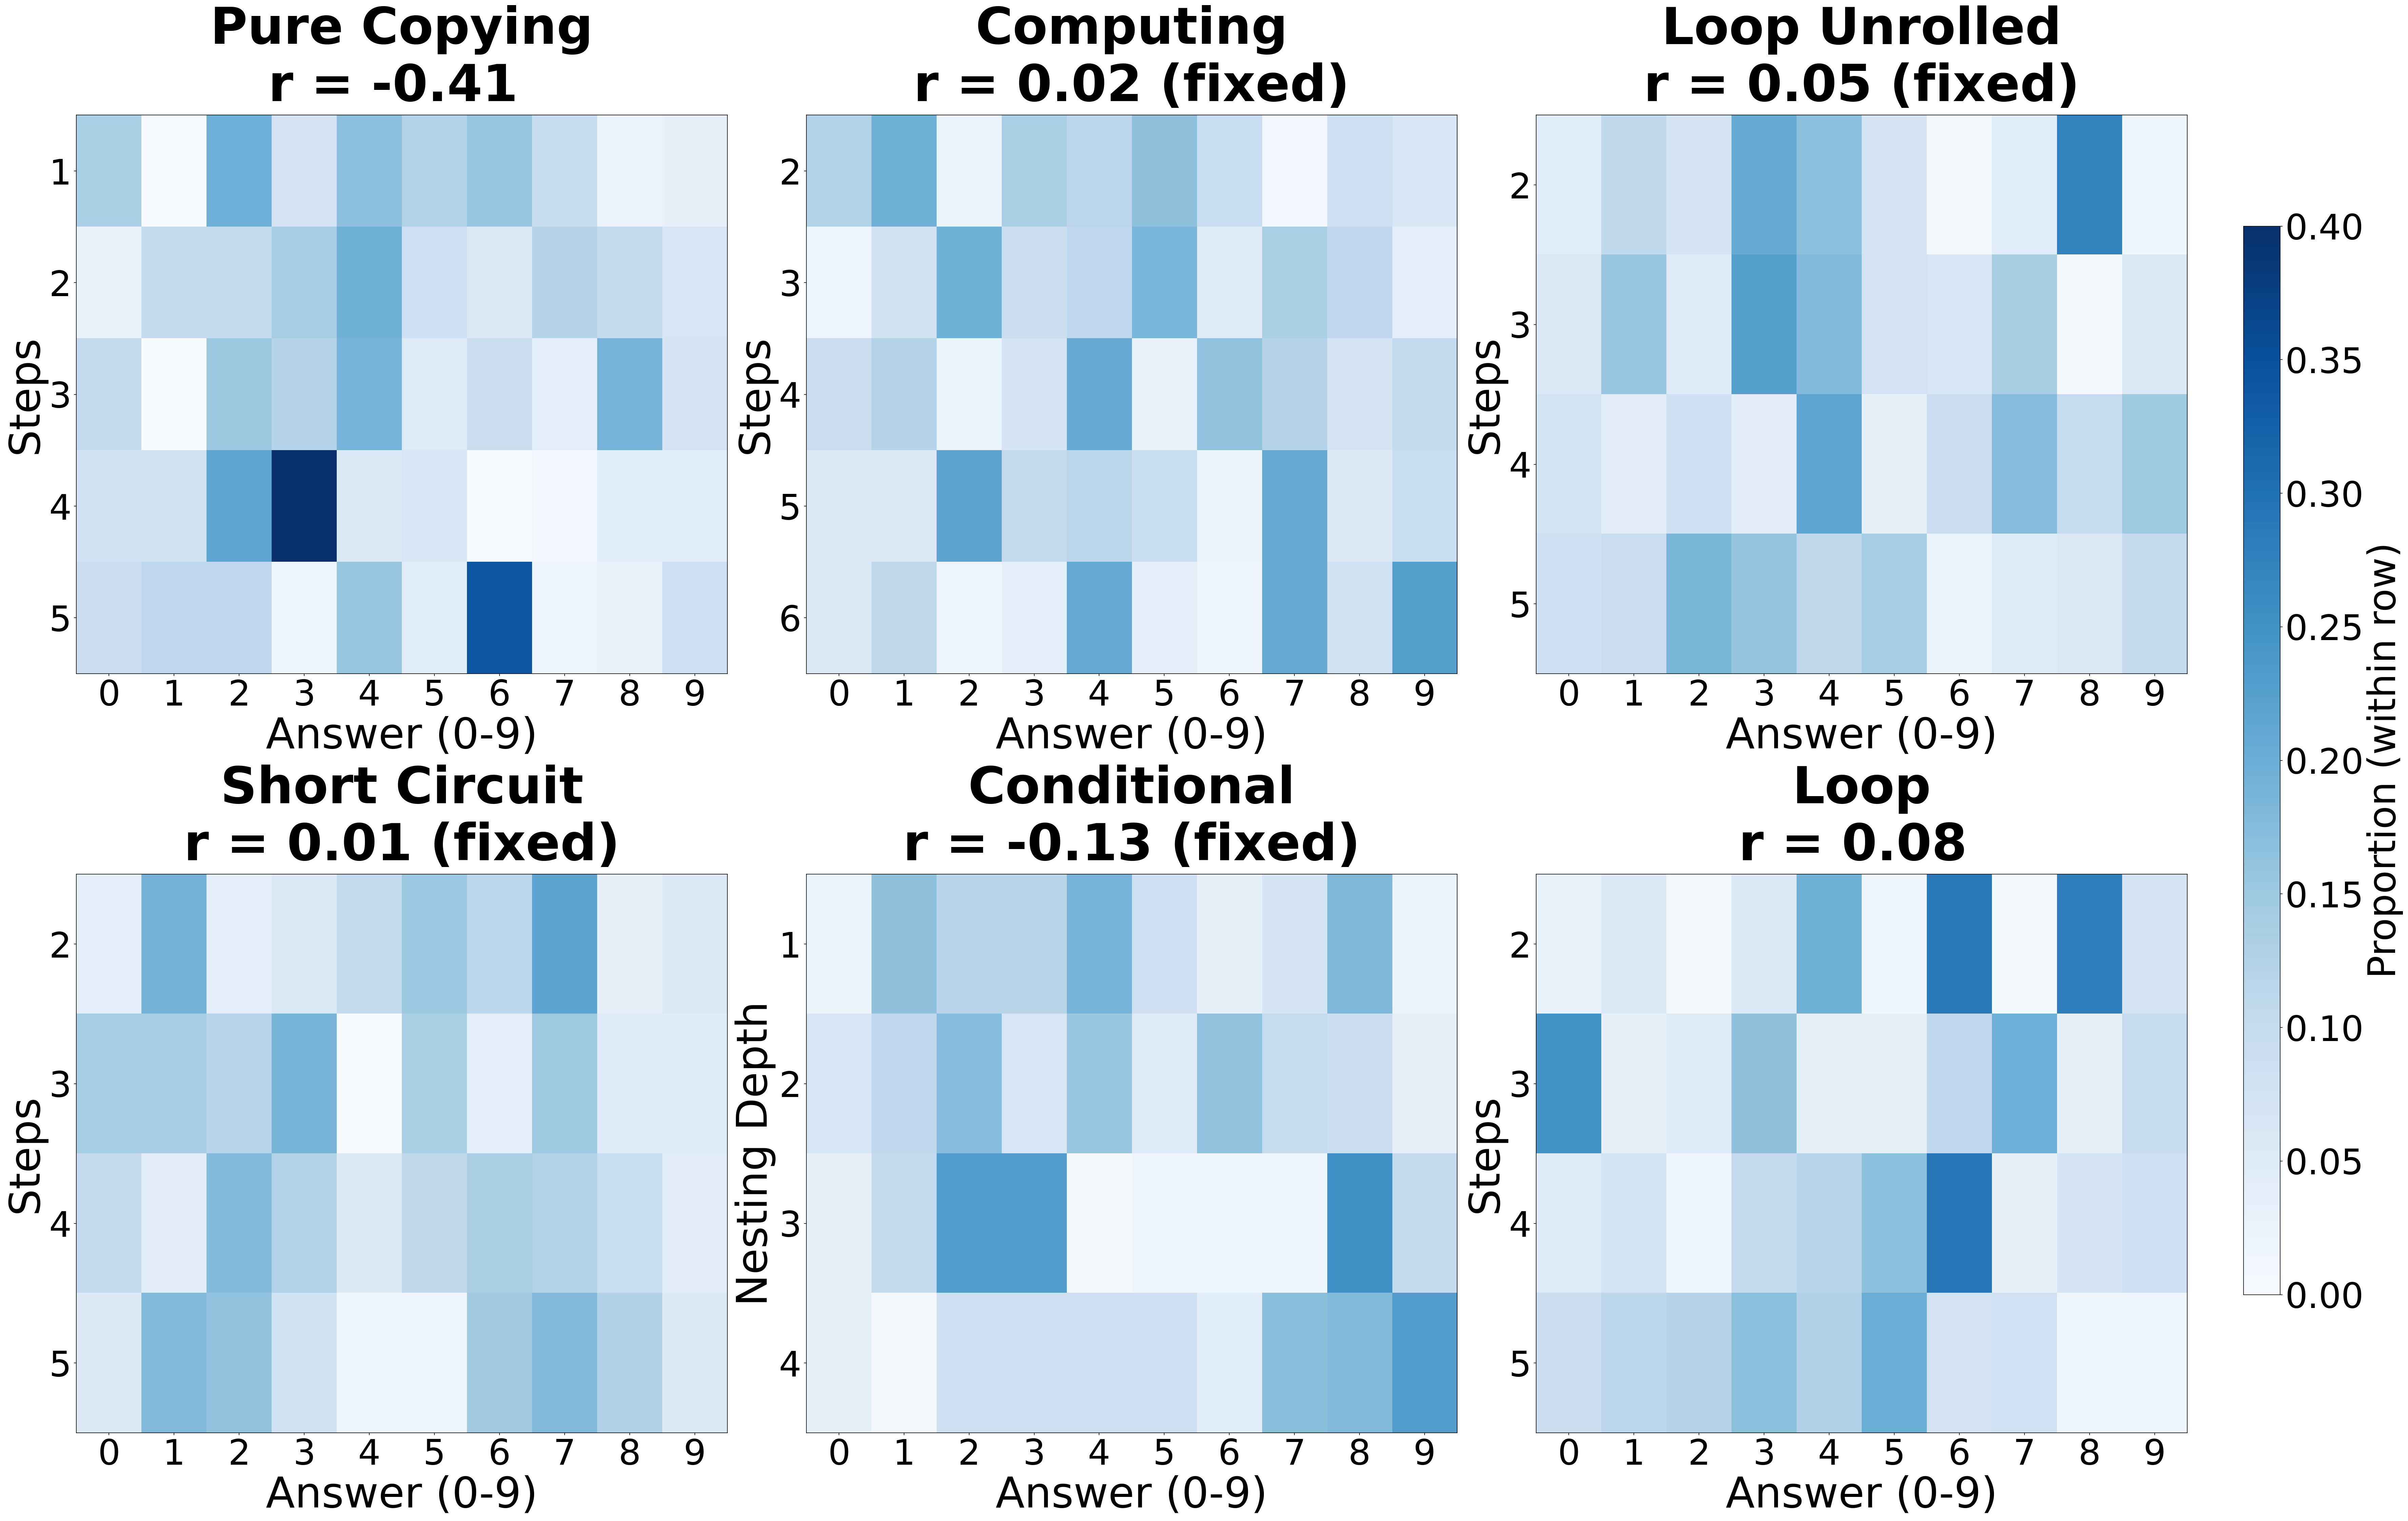
\includegraphics[width=\columnwidth]{figures/appendix/B_answer_distribution.png}
\caption{Answer distributions across control variables for all six tasks. Low Pearson correlations ($|r| < 0.15$ for debiased tasks) suggest that, after debiasing, difficulty parameters are not strongly associated with answer values.}
\label{fig:answer_dist}
\end{figure}
